%----------------------------------------------------------
\def\notedate{2022.06.17}
\def\currentauthor{Амелькина А.-М. (РК6)}
%----------------------------------------------------------
\notestatement{rndhpcrpc}{Удаленный запуск кода Waleffe_flow.Fortran}
%----------------------------------------------------------

\subsubsection{Описание структуры программы Waleffe_flow.Fortran}
Структура директорий исходных кодов и запусков программы Waleffe\_flow.Fortran изображена на рисунке \ref{structure}.
\begin{figure}[!ht]
	\centering
	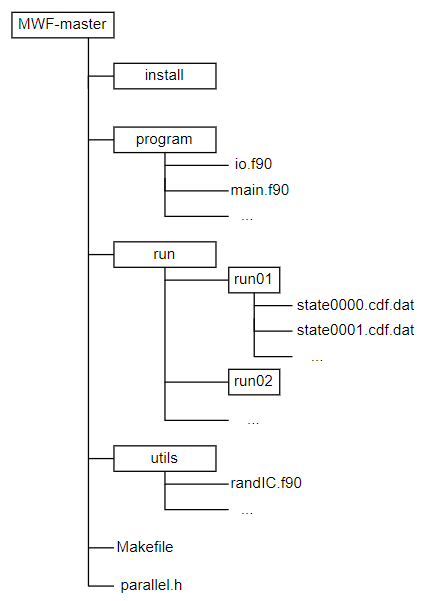
\includegraphics[width=0.45\textwidth]{ResearchNotes/rndcmp_not_rcs_2022_06_17/MWF-иерархия.png}
	\caption{Структура программы Waleffe\_flow.Fortran}\label{structure}
\end{figure} 

%----------------------------------------------------------
\subsubsection{Удаленный запуск кода}

Для подключения к удаленной машине используется SSH -- сетевой протокол прикладного уровня, позволяющий производить удалённое управление операционной системой и туннелирование TCP-соединений  \cite{ssh}.

Для запуска программы Waleffe\_flow.Fortran на удаленной машине необходимо выполнить следующие команды:
\begin{enumerate}
    \item Подключение к удаленной машине \cite{ssh-comand}:
            \begin{verbatim}
            ssh user@server  \end{verbatim}
        В данной работе использовалась виртуальная машина с именем hpc.rk6.bmstu.ru и пользователь amamelkina, поэтому команда выглядела следующим образом: \begin{verbatim}
            ssh amamelkina@hpc.rk6.bmstu.ru   \end{verbatim}
    \item Переход в директорию с программой  \cite{ubuntu-comand}:
            \begin{verbatim}
            cd /home/amamelkina/MWF-master    \end{verbatim}
    \item Чтобы настроить среду для использования библиотек MPI, нужно загрузить соответствующий модуль окружающей среды:
            \begin{verbatim}
            module load mpi \end{verbatim}
    \item Сборка:
            \begin{verbatim}
            make
            make install    \end{verbatim}
    \item Создание начальных условий: \label{IC}
            \begin{verbatim}
            make util
            ./randIC.out    \end{verbatim}
    \item Далее необходимо создать папку, в которую будут записываться результаты. Такие наборы результатов хранятся в папке run. В папке run создается папка с номером (например run10), в нее копируются файлы /install/main.info, /install/main.out. Файл state0000.cdf.dat, полученный в результате выполнения пункта \ref{IC}, должен быть переименован в state.cdf.in и тоже скопирован в новую папку результатов.
    \item Затем нужно перейти в созданную папку и запустить программу:
            \begin{verbatim}
            ./main.out    \end{verbatim}
    \item После остановки программы, когда будет получено необходимое количество данных, можно отключаться от удаленной машины с помощью команды:
            \begin{verbatim} 
            exit \end{verbatim}
    \item Последний шаг -- скопировать результат с удаленной машины на локальную \cite{ssh-cp}:
            \begin{verbatim}
            scp -r user@server:<адрес/откуда/копируем>
                               <адрес/куда/копируем>  \end{verbatim}
\end{enumerate}

Видно, что запуск данной программы на удаленной машине требует выполнения множества команд. Упростим запуск до одной команды -- запуска python-скрипта, в котором будет реализован процесс удаленного запуска.

%----------------------------------------------------------
\subsubsection{Программная реализация}

Для реализации необходимого python-скрипта была использована библиотека fabric. Fabric – это библиотека Python и инструмент командной строки для оптимизации использования SSH для развертывания приложений или задач системного администрирования \cite{fabric-doc}.

Для работы с fabric первым делом нужно создать fabfile и разместить в структуре файлов так, как показано на рисунке \ref{structure_fab}.
\begin{figure}[!ht]
	\centering
	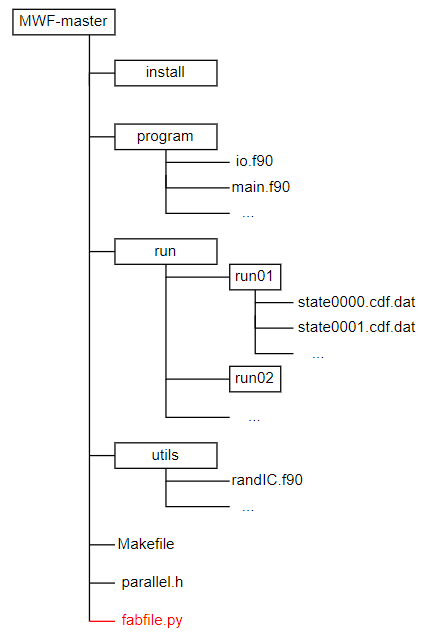
\includegraphics[width=0.45\textwidth]{ResearchNotes/rndcmp_not_rcs_2022_06_17/MWF-иерархия_fab.png}
	\caption{Размещение fabfile}\label{structure_fab}
\end{figure} 

Fabfile -- это то, что контролирует то, что выполняет fabric. Он называется fabfile.py и запускается командой fab. Все функции, определенные в этом файле, будут отображаться как подкоманды fab. Они выполняются на одном или нескольких серверах. Эти серверы могут быть определены либо в fabfile, либо в командной строке \cite{fabric-fab}.

Добавим сервер в fabfile, определив его в переменной окружения env (листинг \ref{host}) \cite{fabric-env}. 
\begin{lstlisting}[label=host, language=Python, caption=Добавление сервера в переменную окружения env] 
        env.hosts = ['hpc.rk6.bmstu.ru']
\end{lstlisting}

Fabric по умолчанию использует локальное имя пользователя при подключении SSH, но при необходимости его можно переопределить, используя env.user. Предоставим пользователю программы возможность ввести имя (листинг \ref{user}). Это реализовано с помощью функции prompt(text, default='', ...) \cite{fabric-func}.
Данная функция выдаёт пользователю запрос с текстом text и возвращает полученное значение. Для удобства к text будет добавлен одиночный пробел.
Если передан параметр default, то он будет выведен в квадратных скобках и будет использоваться в случае, если пользователь ничего не введёт (т.e. нажмёт Enter без ввода текста). По умолчанию значением default является пустая строка.
\begin{lstlisting}[label=user, language=Python, caption=Добавление имени пользователя в переменную окружения env] 
        user = prompt("Enter username", default=’amamelkina’)
        env.user = user
\end{lstlisting}

Также пользователю нужно ввести время в секундах, в течение которого будет выполняться программа.

Затем с помощью функции run(command, ...), которая запускает команду оболочки на удалённом узле, выполняется запуск программы Waleffe\_flow.Fortran.

Также используются функции put(local\_path=None, remote\_path=None, ...) и get(remote\_path, local\_path = None) для загрузки файлов на удаленный сервер и скачивания файлов с удалённого сервера соответственно.

Листинг кода python-скрипта представлен в Приложении.

Для запуска fabric предоставляет команду fab, которая считывает свою конфигурацию из файла fabfile.py.

В листинге \ref{hello} представлена простая функция, с помощью которой будет продемонстрировано, как использовать fabric \cite{fabric-hello}. Эта функция сохранена как fabfile.py в текущем рабочем каталоге.
\begin{lstlisting}[label=hello, language=Python, caption=Пример функции]
        def hello():
            print("Hello!")
\end{lstlisting}

 Функция приветствия может быть выполнена с помощью fab инструмента следующим образом:
\begin{verbatim}
        fab hello
\end{verbatim}

В результате выполнения этой команды будет выведено "Hello!".

Таким образом, для запуска программы Waleffe\_flow.Fortran на удаленной машине теперь необходимо выполнить только одну команду:
\begin{verbatim}
        fab run_fortran
\end{verbatim}

В результате работы данного python-скрипта на персональном компьютере в папке run появится новая папка с результатами запуска.

%----------------------------------------------------------
% Атрибуты задачи
\noteattributes{}
%----------------------------------------------------------
